% !TeX spellcheck = <none>
%!TEX root = Projeto.tex

\subsection{Processo de renderização do documento web}
Para que seja visualizada no navegador, o conteúdo da página web passa pelo processo de renderização implementado pelo mecanismo de visualização. Nesse processo, o navegador leva em consideração características ambientais como a resolução do dispositivo gráfico, o tamanho do \poe{viewport} (janela do navegador), o tipo de dispositivo de saída (tela, impressora) e os recursos de sistema disponíveis (taxa de utilização da CPU, do processador gráfico e da memória RAM), e também definições da página web como o conjunto de folhas de estilo, recursos audiovisuais incorporados (imagens, vídeos) e o próprio conteúdo textual codificado em marcação HTML. Dado que quaisquer dessas características pode variar durante o ciclo de vida de uma página web, o navegador pode repetir o processo de renderização diversas vezes em resposta a essas variações.

\citeinline{Google2018_Rendering}, ao descrever o processo de renderização implementado pelo navegador Chrome, menciona duas etapas iniciais: a construção da árvore de objetos do HTML, resultando na estrutura DOM, e a construção da árvore de definições de CSS, resultando na estrutura CSSOM. Ambas as estruturas são independentes entre si, mas sua combinação tem efeito sobre a terceira etapa da renderização, responsável por construir a árvore de visualização (\poe{render tree}) da página web.

A árvore de visualização fornece ao navegador a informação necessária para a definição do \poe{layout} de cada elemento HTML em função da visibilidade, das dimensões e do estilo de cada elemento. O \poe{layout} é um dado de entrada para o processo de desenho que gera \poe{pixels} visíveis no dispositivo de saída. Uma síntese desse processo é enumerada por \citeinline{Google2018_Rendering} nos seguintes passos, ilustrados pelo diagrama \ref{Fig: renderTreeCtor}:

\begin{alineas}
	\item O DOM e o CSSOM são combinados na árvore de visualização;
	%\item A árvore de visualização contém apenas os nós necessários para a apresentação da página;
	\item É calculado o \poe{layout} -- tamanho, posição e estilo -- de cada elemento;
	\item Elementos sem \poe{layout} são descartados da árvore;
	\item Os nós da árvore de visualização são desenhados no dispositivo de saída.
\end{alineas}

\begin{figure}[h]
	\centering
	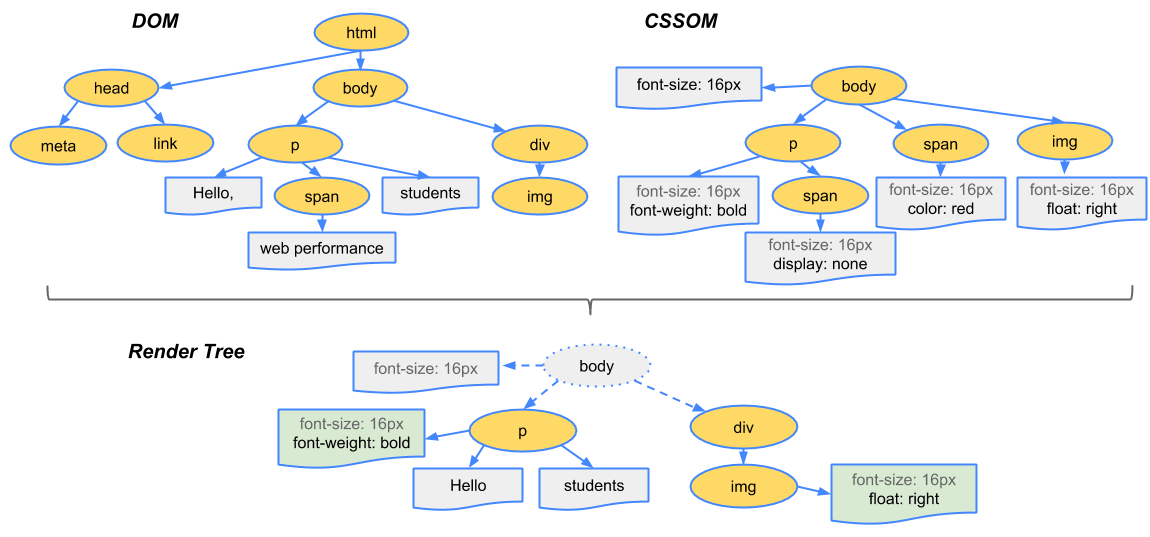
\includegraphics[width=\textwidth]{diagramas/render-tree-construction.png}
	\label{Fig: renderTreeCtor}
	\caption[Construção da árvore de visualização do navegador]{Construção da árvore de visualização do navegador \cite{Google2018_Rendering}}
\end{figure}


\subsubsection{Conflitos de regras em CSS}
A estrutura CSSOM deriva da combinação das regras (\poe{style rules}) de todas as folhas de estilo incorporadas pela página. A existência de um CSSOM único pode desencadear efeitos colaterais como a colisão de nomes de regras (simultaneamente definidas em folhas de estilo concorrentes) e a herança inesperada de atributos de estilo, ambos levando a \poe{layouts} diferentes daquele esperado pelo desenvolvedor de uma página web. O diagrama \ref{Fig: cssomConflict} exemplifica esses efeitos.

\begin{figure}[h]
	\centering
	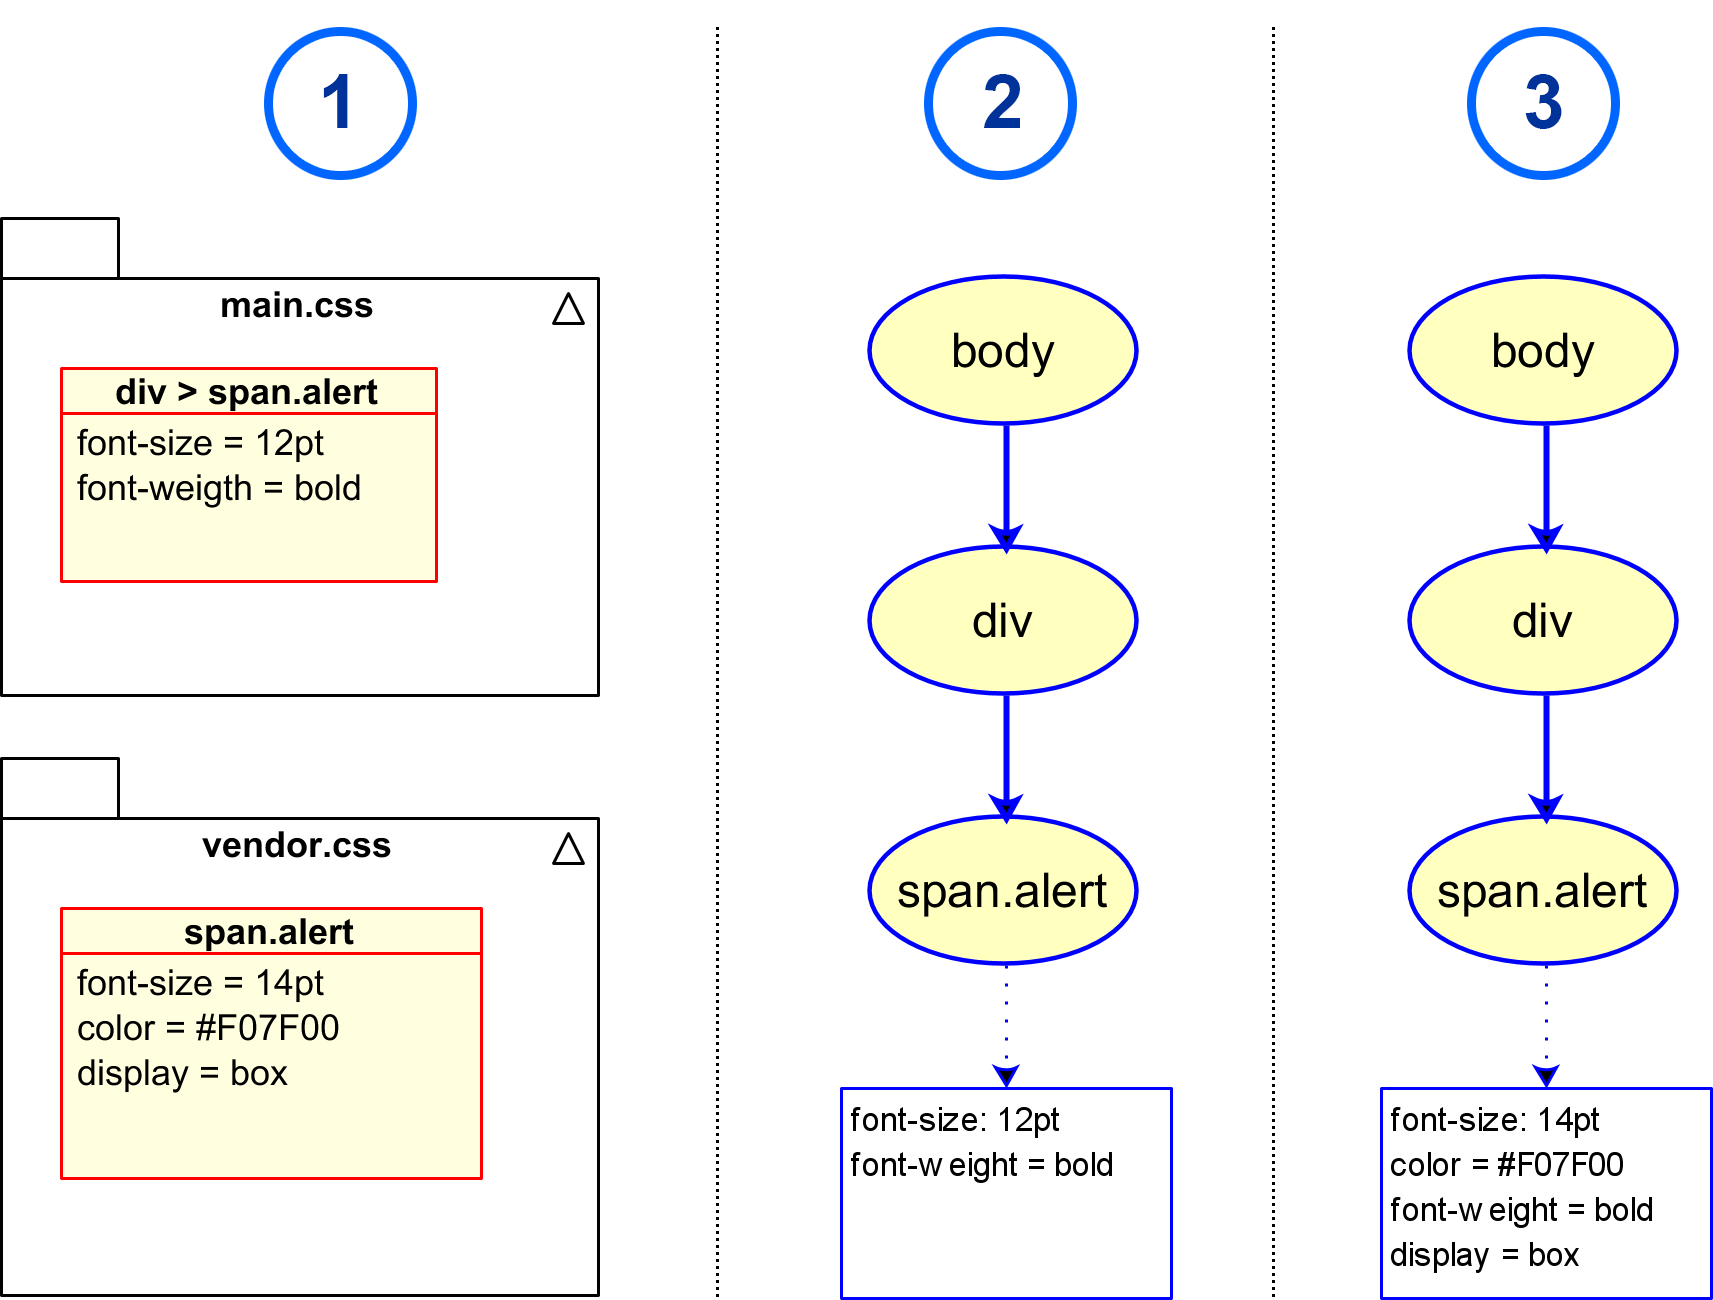
\includegraphics[width=12cm]{diagramas/conflito-CSSOM.png}
	\label{Fig: cssomConflict}
	\caption[Conflito de regras em folhas de estilo]{Conflito de regras em folhas de estilo. Sob \circled{1}, duas folhas de estilo independentes, \textbf{main.css} e \textbf{vendor.css}, são incorporadas a uma mesma página. O desenvolvedor da página não tem controle sobre \textbf{vendor.css}, que inadvertidamente redefine a regra de estilos aplicável aos elementos \textbf{span} decorados com a classe \textbf{alert}. Com isso, a estrutura CSSOM pretendida pelo desenvolvedor da página, sob \circled{2}, é calculada de modo a produzir um layout divergente, ilustrado pela estrutura CSSOM sob \circled{3}.}
\end{figure}

Como o meacnismo de visualização é tolerante aos conflitos de especificação de regras de estilo, as soluções para os efeitos colaterais decorrentes é paliativa. Os desenvolvedores são encorajados a estabelecer ``espaços de nome'' que delimitem o escopo de aplicação das regras de estilo\footnote{``Defensive HTML and CSS'' -- \url{https://www.webdesignerdepot.com/2013/04/defensive-html-and-css/}}, diminuindo a chance de que as árvores CSSOM resultantes contenham nós conflitantes. No entanto, uma proposta mais robusta, inaugurada pela padronização de \poe{shadow DOMs}, pode ser empregada com o propósito de isolar árvores de CSSOM e, consequentemente, produzir árvores de visualização independentes.


\subsubsection{Isolamento de árvores de visualização com \poe{Shadow DOM}}
\label{Section: introShadowDOM}

\dubious{CONTINUAR DEPOIS. Falar sobre os conceitos: shadow host, shadow tree. Não falar sobre: modos open e closed.}

A proposta do mecanismo de Shadow DOM \cite{W3C:ShadowDOM} é definir uma forma padronizada para que o próprio navegador minimize as interferências entre componentes de página que, de outra forma, poderiam causar as já mencionadas colisões de regras de estilos e \scripts{}. A utilização de Shadow DOMs faz com que o modelo de objetos em uma página isole determinadas regiões do DOM em \textit{shadow roots} completamente independentes.

Shadow DOM, \dubious{proposta em xx/201x,} é implementada pelos navegadores Chrome, Opera e Safari, com suporte planejado para os navegadores Firefox e Microsoft Edge \dubious{para os próximos meses}.
